\usepackage[spanish]{babel}
\usepackage[ansinew]{inputenc}
\usepackage{amsmath}
\usepackage{enumerate}
\usepackage{latexsym}
\usepackage[noend]{algorithmic}
\usepackage{algorithm}

\title{Archivos y Streams}
\author{Algoritmos y Estructuras de Datos \\
Programaci�n Estructurada}
\date{}

\newcommand{\pseudohrule}{\vskip 5pt \hrule}

\newenvironment{pseudo}[1][\normalsize]{
\begin{figure}
#1
\begin{semiverbatim}
}{
\end{semiverbatim}
\normalsize
\end{figure}
}

\setlength{\parskip}{3pt plus 1pt minus 1pt}

\begin{document}

\begin{frame}
\titlepage
\end{frame}

%%%%%%%%%%%%%%%%%%%%%%%%%%

\begin{frame}[fragile]{Repaso}

\begin{block}<1->{Algoritmo}
Un algoritmo es una lista de finita intrucciones que permiten hallar la soluci�n a un problema.
\end{block}

\begin{block}<2->{Especificaci�n}
La especificaci�n de un algoritmo es un contrato entre el programador y el usuario en donde se definen 
cuales son los datos de entrada, la precondici�n y la postcondici�n del mismo.
\end{block}

\end{frame}

%%%%%%%%%%%%%%%%%%%%%%%%%%

\begin{frame}[fragile]{Repaso}

\begin{block}<1->{Correctitud}
Un algoritmo es correcto cuando siempre que vale la precondici�n podemos asegurar que el programa termina y la postcondici�n se cumple.
\end{block}

\begin{block}<2->{Tipo de Dato}
Un tipo de dato es la implementaci�n de un concepto de la vida real.
\end{block}

\end{frame}

%%%%%%%%%%%%%%%%%%%%%%%%%%

\begin{frame}[fragile]{Archivos}

\begin{block}{Qu� es un archivo?}
Un archivo es una colecci�n de informaci�n guardada en la computadora. Hay distintos tipos de archivos, que contienen distinto tipo de informaci�n. Los tipos de archivo muchas veces se identifican por su extensi�n. Por ejemplo:
\begin{itemize}
\item Un archivo de texto plano (txt)
\item Un archivo de Word (doc)
\item Un archivo ejecutable o programa (exe)
\item Un archivo de c�digo python (py)
\end{itemize}
\end{block}

\end{frame}

%%%%%%%%%%%%%%%%%%%%%%%%%%

\begin{frame}[fragile]{En el fondo...}

M�s all� del tipo de archivo, en el fondo todos los archivos no son m�s que secuencias de ceros y unos:

\[
10101010101110101010101010101010101010101010...
\]

Lo que cambia es c�mo interpretamos la informaci�n representada en esos ceros y unos. Cuando los interpretamos como texto, decimos que se trata de un \textit{archivo de texto plano}. Si no, hablamos de un \textit{archivo binario}.

\end{frame}

%%%%%%%%%%%%%%%%%%%%%%%%%%

\begin{frame}[fragile]{Streams}

Un \textbf{stream} es una secuencia de datos que se va consumiendo o escribiendo a medida que pasa el tiempo. Es la manera m�s frecuente en la que se leen o escriben datos desde un programa. 

\begin{itemize}
\item Stream de entrada: permite leer datos desde el programa
\item Stream de salida: permite escribir datos a un destino externo
\end{itemize}

Un ejemplo sencillo de stream de salida es la consola. Cada vez que hacemos \texttt{print} o usamos \texttt{cout} estamos escribiendo datos al stream est�ndar de salida del programa.

Asimismo, cada vez que el usuario ingresa algo por consola, usando \texttt{raw\_input} o \texttt{cin}, estamos consumiendo el stream est�ndar de entrada.

\end{frame}

%%%%%%%%%%%%%%%%%%%%%%%%%%

\begin{frame}[fragile]{Archivos como Streams}

Cuando queremos leer de un archivo, lo podemos acceder como si este fuera un stream de datos. El stream tiene una posici�n actual que indica en qu� parte del archivo estamos, y podemos avanzarlo para leer secuencialmente los datos.

De esta forma, la lectura de un archivo puede hacerse de la siguiente manera:

\begin{pseudo}
streamLectura = abrirArchivo('miarchivo.txt')
para cada letra en streamLectura
  mostrar letra por pantalla
fin
cerrar streamLectura
\end{pseudo}

\end{frame}

%%%%%%%%%%%%%%%%%%%%%%%%%%

\begin{frame}[fragile]{Leyendo el archivo}

Una vez abierto el archivo como un stream de datos para leerlo, podemos recorrerlo de varias maneras. Distintos lenguajes proveen distintos m�todos para leer el archivo, siempre avanzando el stream. Por ejemplo, podemos leer caracter por caracter:

\begin{center}
\begin{figure}
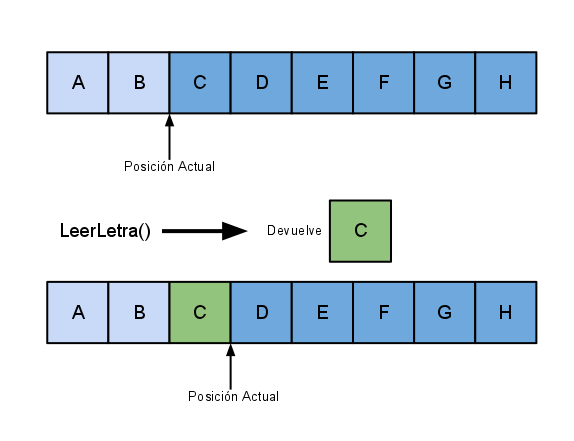
\includegraphics[scale=0.4]{C14/FileRead.png}
\end{figure}
\end{center}

\end{frame}

%%%%%%%%%%%%%%%%%%%%%%%%%%

\begin{frame}[fragile]{Escribiendo en el archivo}

Del mismo modo, podemos abrir un archivo como un stream de datos de salida, para escribirlo. Esto nos permite enviar datos al stream, tal como lo hac�amos al escribir en pantalla, pero para que ahora se escriban en el archivo.

\begin{pseudo}
streamEscritura = abrirArchivo('miarchivo.txt', 'escribir')
streamEscritura.escribir('Hola ')
streamEscritura.escribir('mundo!')
cerrar streamEscritura
\end{pseudo}

\uncover<2->{
Al terminar la ejecuci�n, el contenido de \texttt{miarchivo.txt} ser�:
\vskip 5pt
\texttt{Hola mundo!}

}

\end{frame}

%%%%%%%%%%%%%%%%%%%%%%%%%%

\begin{frame}[fragile]{Cerrar el stream!}

Es muy importante siempre acordarse de \textit{cerrar el stream}! 

Cuando cerramos el stram estamos indicando que ya no vamos a usar m�s el archivo, y le permitimos a otro programa que pueda modificarlo. Adem�s nos aseguramos que cualquier escritura que hubiera quedado pendiente sea persistida efectivamente en el archivo.

\end{frame}

%%%%%%%%%%%%%%%%%%%%%%%%%%

\begin{frame}[fragile]{Resumiendo}

\begin{itemize}
\item Un archivo es un bloque de informaci�n en disco en la computadora
\item Un stream es una secuencia de datos que podemos leer o escribir
\item Desde nuestros programas vamos a acceder a los archivos como streams: usando m�todos para leer secuencialmente o ir escribiendo lo necesario
\item Es importante siempre cerrar el stream a un archivo para indicar que se termin� de usarlo
\end{itemize}

\end{frame}

\end{document}



